\subsection{La notation de la batterie}
\subsubsection{La hauteur des notes et les têtes de notes}
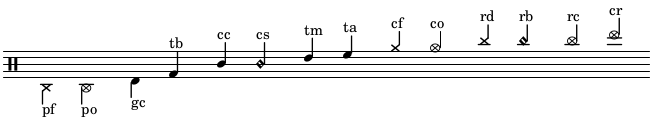
\includegraphics[height=30mm, width=155mm]{z_images/1_description_notation/notes.png}
partition 1
\subsubsection{Les nuances}
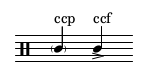
\includegraphics[height=20mm, width=35mm]{z_images/1_description_notation/nuances.png}\\
partition 2
\subsubsection{La séparation des voix}
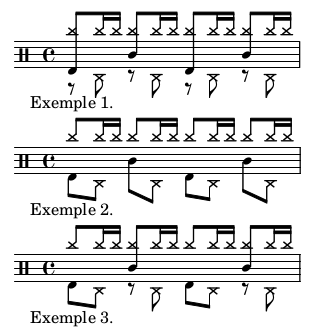
\includegraphics[height=65mm, width=60mm]{z_images/1_description_notation/separation/0_exemples_separation.png}\\
partition 3
\subsection{La notation midi de la batterie}
\subsubsection{Les pitchs et la vélocité}
\begin{table}[h]
	\centering
	\begin{tabular}{|c|c|c|} \hline
		Codes & Instruments & Pitchs \\ \hline
		pf & charley-pied-fermé & 44 \\
		po & charley-pied-ouvert & ? \\
		gc & grosse-caisse & 36 \\
		tb & tom-basse & 43, 58 \\
		cc & caisse-claire & 38, 40 \\
		cs & cross-stick & 37 \\
		tm & tom-medium & 45, 47 \\
		ta & tom-alto & 48, 50 \\
		cf & charley-main-fermé & ? \\
		co & charley-main-ouvert & 26 \\
		rd & ride & 51 \\
		rb & ride-cloche (bell) & 53 \\
		rc & ride-crash & 59 \\
		cr & crash & 55 \\ \hline
	\end{tabular}
	\caption{Pitchs et instruments}
	%	\label{tab:exemple}
\end{table}
\begin{table}[h]
	\centering
	\begin{tabular}{|c|c|c|c|} \hline
		Codes & Instruments & Pitchs & Vélocité \\ \hline
		cop & charley-main-ouvert & 46 & ? \\ \hline
	\end{tabular}
	\caption{Vélocité et nuances}
\end{table}
Nous ne prendrons en compte la vélocité que pour la cc, les toms et les cymbales jouées aux mains. Les nuances de grosse caisse et charley aux pieds sont le plus souvent insignifiants, elles ne sont marquées sur le figure qu’à titre indicatif.\\\\
Si la vélocité est en dessous de 40, il s’agit de ghost-notes : la tête de note devra être entouré de parenthèses et le suffixe \textit{p (piano)} devra être ajouté au codes de l’instrument. (Voir ccp ci-dessus.)\\\\
Si la vélocité est au dessus de 90, il s’agit de notes accentuées : le symbole « > » et le suffixe \textit{f (forte)} devra être ajouté au codes de l’instrument. (Voir ccf ci-dessus.)\\\\
Lorsque la vélocité va de 40 à 89, on considèrera le volume comme normal et aucun symbole supplémentaire ne sera ajouté à la note.\\\\
L’instrument qui sera difficile à placer sera la caisse claire car elle ne sera pas toujours affiliée aux mêmes instruments.
\subsubsection{Les dilemmes}
Le charley de pitch 46 est considéré comme le charley ouvert joué à la main sur le haut de la cymbale mais souvent, ça correspond au geste « tranche-olive » de la baguette lorsque le batteur accentue avec la tranche et joue moins fort avec l’olive sur le plat de la cymbale. Je vais dans un premier temps considérer le pitch comme \textbf{charley-main-ouvert-piano} (ghost-note)
\newpage
\subsubsection{Représentations en arbres}
Voici une représentation de la \textit{partition 3} en arbre de rythme avec les codes de chaque instrument :\\\\
\Tree[ [ [rd\\gc ][ [rd\\pf ][rd ]]]
[ [rd\\cc ][ [rd\\pf ][rd ]]]
[ [rd\\gc ][ [rd\\pf ][rd ]]]
[ [rd\\cc ][ [rd\\pf ][rd ]]] ]\\\\\\
Ci-dessous, le même arbre dont les codes des instruments sont remplacés par leurs données midi respectives :\\\\
\Tree[ [ [51\\36 ][ [51\\44 ][51 ]]]
[ [51\\38 ][ [51\\44 ][51 ]]]
[ [51\\36 ][ [51\\44 ][51 ]]]
[ [51\\38 ][ [51\\44 ][51 ]]] ]\\\\\\
Cet arbre représente un rythme unique dont les possiblités de notation sur une partition sont théoriquement multiples.(Voir \textit{partition 3}).